\chapter{Конструкторская часть}

\section{Требования к программному обеспечению}

Программа должна предоставлять следующий функционал:
\begin{itemize}
    \item изменение параметров направления освещения;
    \item изменение положения камеры в пространстве;
    \item настройка параметров L-системы;
    \item настройка параметров геометрии дерева;
    \item генерация и визуализация дерева, при заданных параметрах L-системы и геометрии дерева.
\end{itemize}

\section{Используемые структуры данных}
Для визуализации трёхмерных деревьев используются следующие структуры данных.
\begin{itemize}
    \item Вершина --- структура для хранения атрибутов одной точки поверхности, содержащая следующие поля:
        \begin{itemize}
            \item координаты положения --- трёхмерный вектор вещественных чисел;
            \item нормаль --- вектор, задающий направление перпендикуляра к поверхности в данной точке.
        \end{itemize}
    \item Треугольник --- структура для описания грани поверхности, содержащая три целочисленных индекса, ссылающихся на вершины в общем списке.
    \item Полигональная сетка --- структура для хранения объекта сцены, содержащая следующие поля:
        \begin{itemize}
            \item список вершин --- массив структур <<вершина>>;
            \item список треугольников --- массив структур <<треугольник>>.
        \end{itemize}
    \item Источник освещения --- структура для хранения направления света в виде трёхмерного векотра и интенсивности.
    \item Камера --- структура, отвечающая за формирование изображения трёхмерной модели. Содержит следующие поля:
        \begin{itemize}
            \item положение камеры --- тройка вещественных чисел, задающая координаты камеры;
            \item точка наблюдения --- тройка вещественных чисел, задающая центр сцены, на который направлен взгляд;
            \item параметры проекции --- угол обзора, соотношение сторон, расстояния до ближней и дальней плоскостей отсечения.
        \end{itemize}
    \item Сцена --- структура, содержащая в себе набор объектов, источник освещения и камеру.
\end{itemize}



\section{Разработка алгоритмов}

\subsection{Функциональная модель процесса построения изображения}

На рисунке~\ref{fig:idef_0} показана диаграмма IDEF0 верхнего уровня, описывающая построение изображения.

На рисунке~\ref{fig:idef_0_1} представлена диаграмма IDEF0 декомпозиции уровня A0.

На рисунке~\ref{fig:idef_0_2} представлена диаграмма IDEF0 декомпозиции уровня A1.

На рисунке~\ref{fig:idef_0_3} представлена диаграмма IDEF0 декомпозиции уровня A2.

На рисунке~\ref{fig:idef_0_4} представлена диаграмма IDEF0 декомпозиции уровня A3.

\begin{figure}[H]
    \centering
    \includegraphics[width=0.95\textwidth]{images/01_A0.pdf}
    \caption{Функциональная схема алгоритма построения изображения,
декомпозиция верхнего уровня}
    \label{fig:idef_0}
\end{figure}

\begin{figure}[H]
    \centering
    \includegraphics[width=0.95\textwidth]{images/02_A0.pdf}
    \caption{Функциональная схема алгоритма построения изображения,
декомпозиция уровня А0}
    \label{fig:idef_0_1}
\end{figure}

\begin{figure}[H]
    \centering
    \includegraphics[width=0.95\textwidth]{images/03_A1.pdf}
    \caption{Функциональная схема алгоритма построения изображения,
декомпозиция уровня А1}
    \label{fig:idef_0_2}
\end{figure}

\begin{figure}[H]
    \centering
    \includegraphics[width=0.95\textwidth]{images/04_A2.pdf}
    \caption{Функциональная схема алгоритма построения изображения,
декомпозиция уровня А2}
    \label{fig:idef_0_3}
\end{figure}

\begin{figure}[H]
    \centering
    \includegraphics[width=0.95\textwidth]{images/05_A3.pdf}
    \caption{Функциональная схема алгоритма построения изображения,
декомпозиция уровня А3}
    \label{fig:idef_0_4}
\end{figure}

\subsection{Алгоритм построения изображения}
Для отображения трехмерной сцены на двумерный экран координаты вершин каждого объекта должны пройти последовательность преобразований из локальной системы координат в систему координат экрана.

Результирующее положение вершины $V_{clip}$ в пространстве отсечения вычисляется по формуле~\eqref{eq:v_clip} путем умножения исходных локальных координат вершины $V_{local}$ на матрицу модели ($M$), матрицу вида ($V$) и матрицу проекции ($P$):

\begin{equation}
    \label{eq:v_clip}
    V_{clip} = P \cdot V \cdot M \cdot V_{local}
\end{equation}


\textbf{Матрица модели ($M$)} преобразует вершины из локальных координат объекта в мировые координаты. Она включает в себя перенос, поворот и масштабирование.

\textbf{Матрица вида ($V$)} преобразует мировые координаты в систему координат камеры. Она определяется положением наблюдателя и направлением взгляда.

\textbf{Матрица проекции ($P$)} преобразует координаты из системы камеры в пространство отсечения, отображая видимую усечённую пирамиду в канонический объём в однородных координатах.


На рисунке~\ref{fig:draw_iamage} представлена схема алгоритма построения изображения.


\begin{figure}[H]
    \centering
    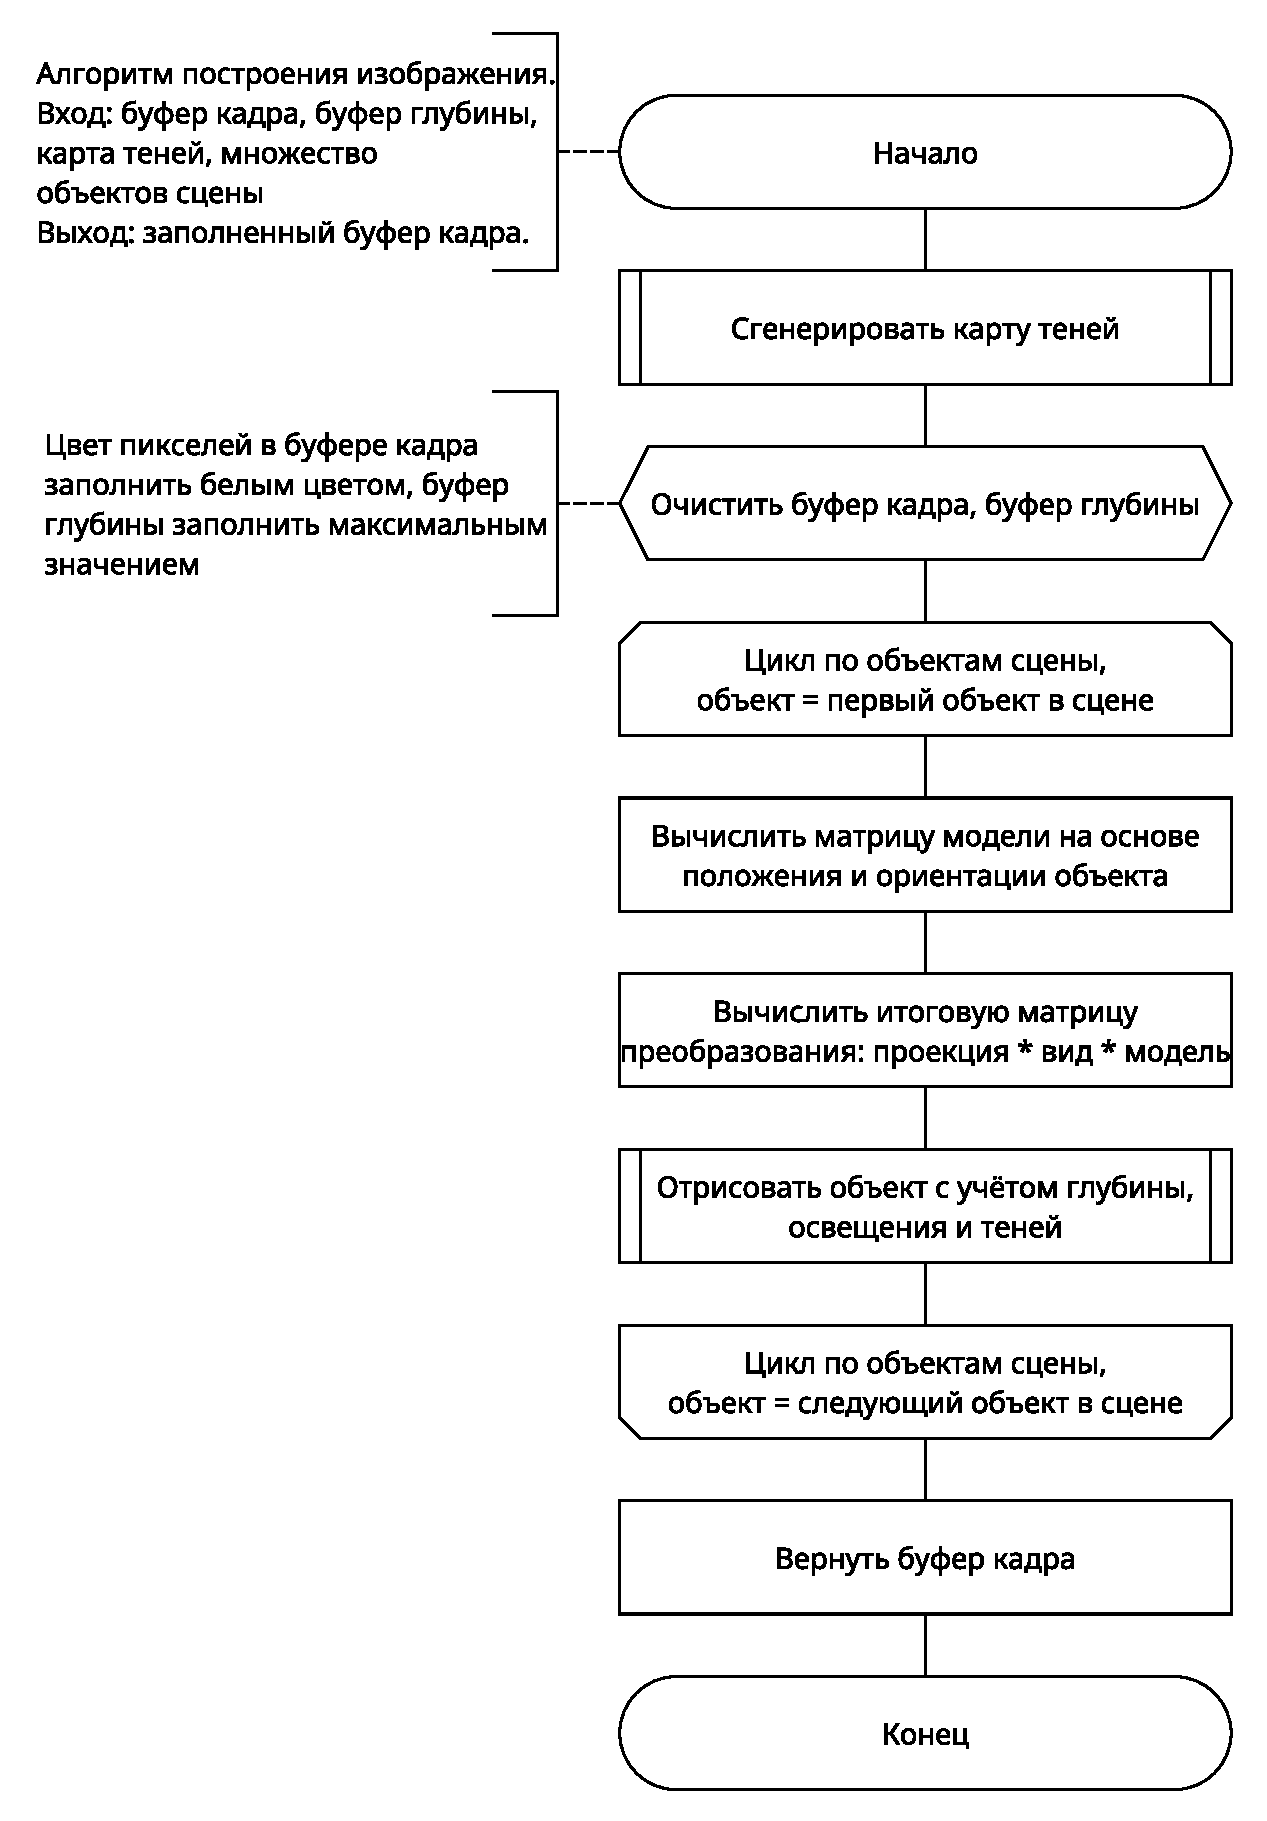
\includegraphics[width=0.9\textwidth]{images/draw_image.pdf}
    \caption{Схема алгоритма построения кадра}
    \label{fig:draw_iamage}
\end{figure}


\subsection{Алгоритм построения карты теней}

На рисунке~\ref{fig:shadow_map} представлена схема алгоритма построения теневой карты.
\begin{figure}[H]
    \centering
    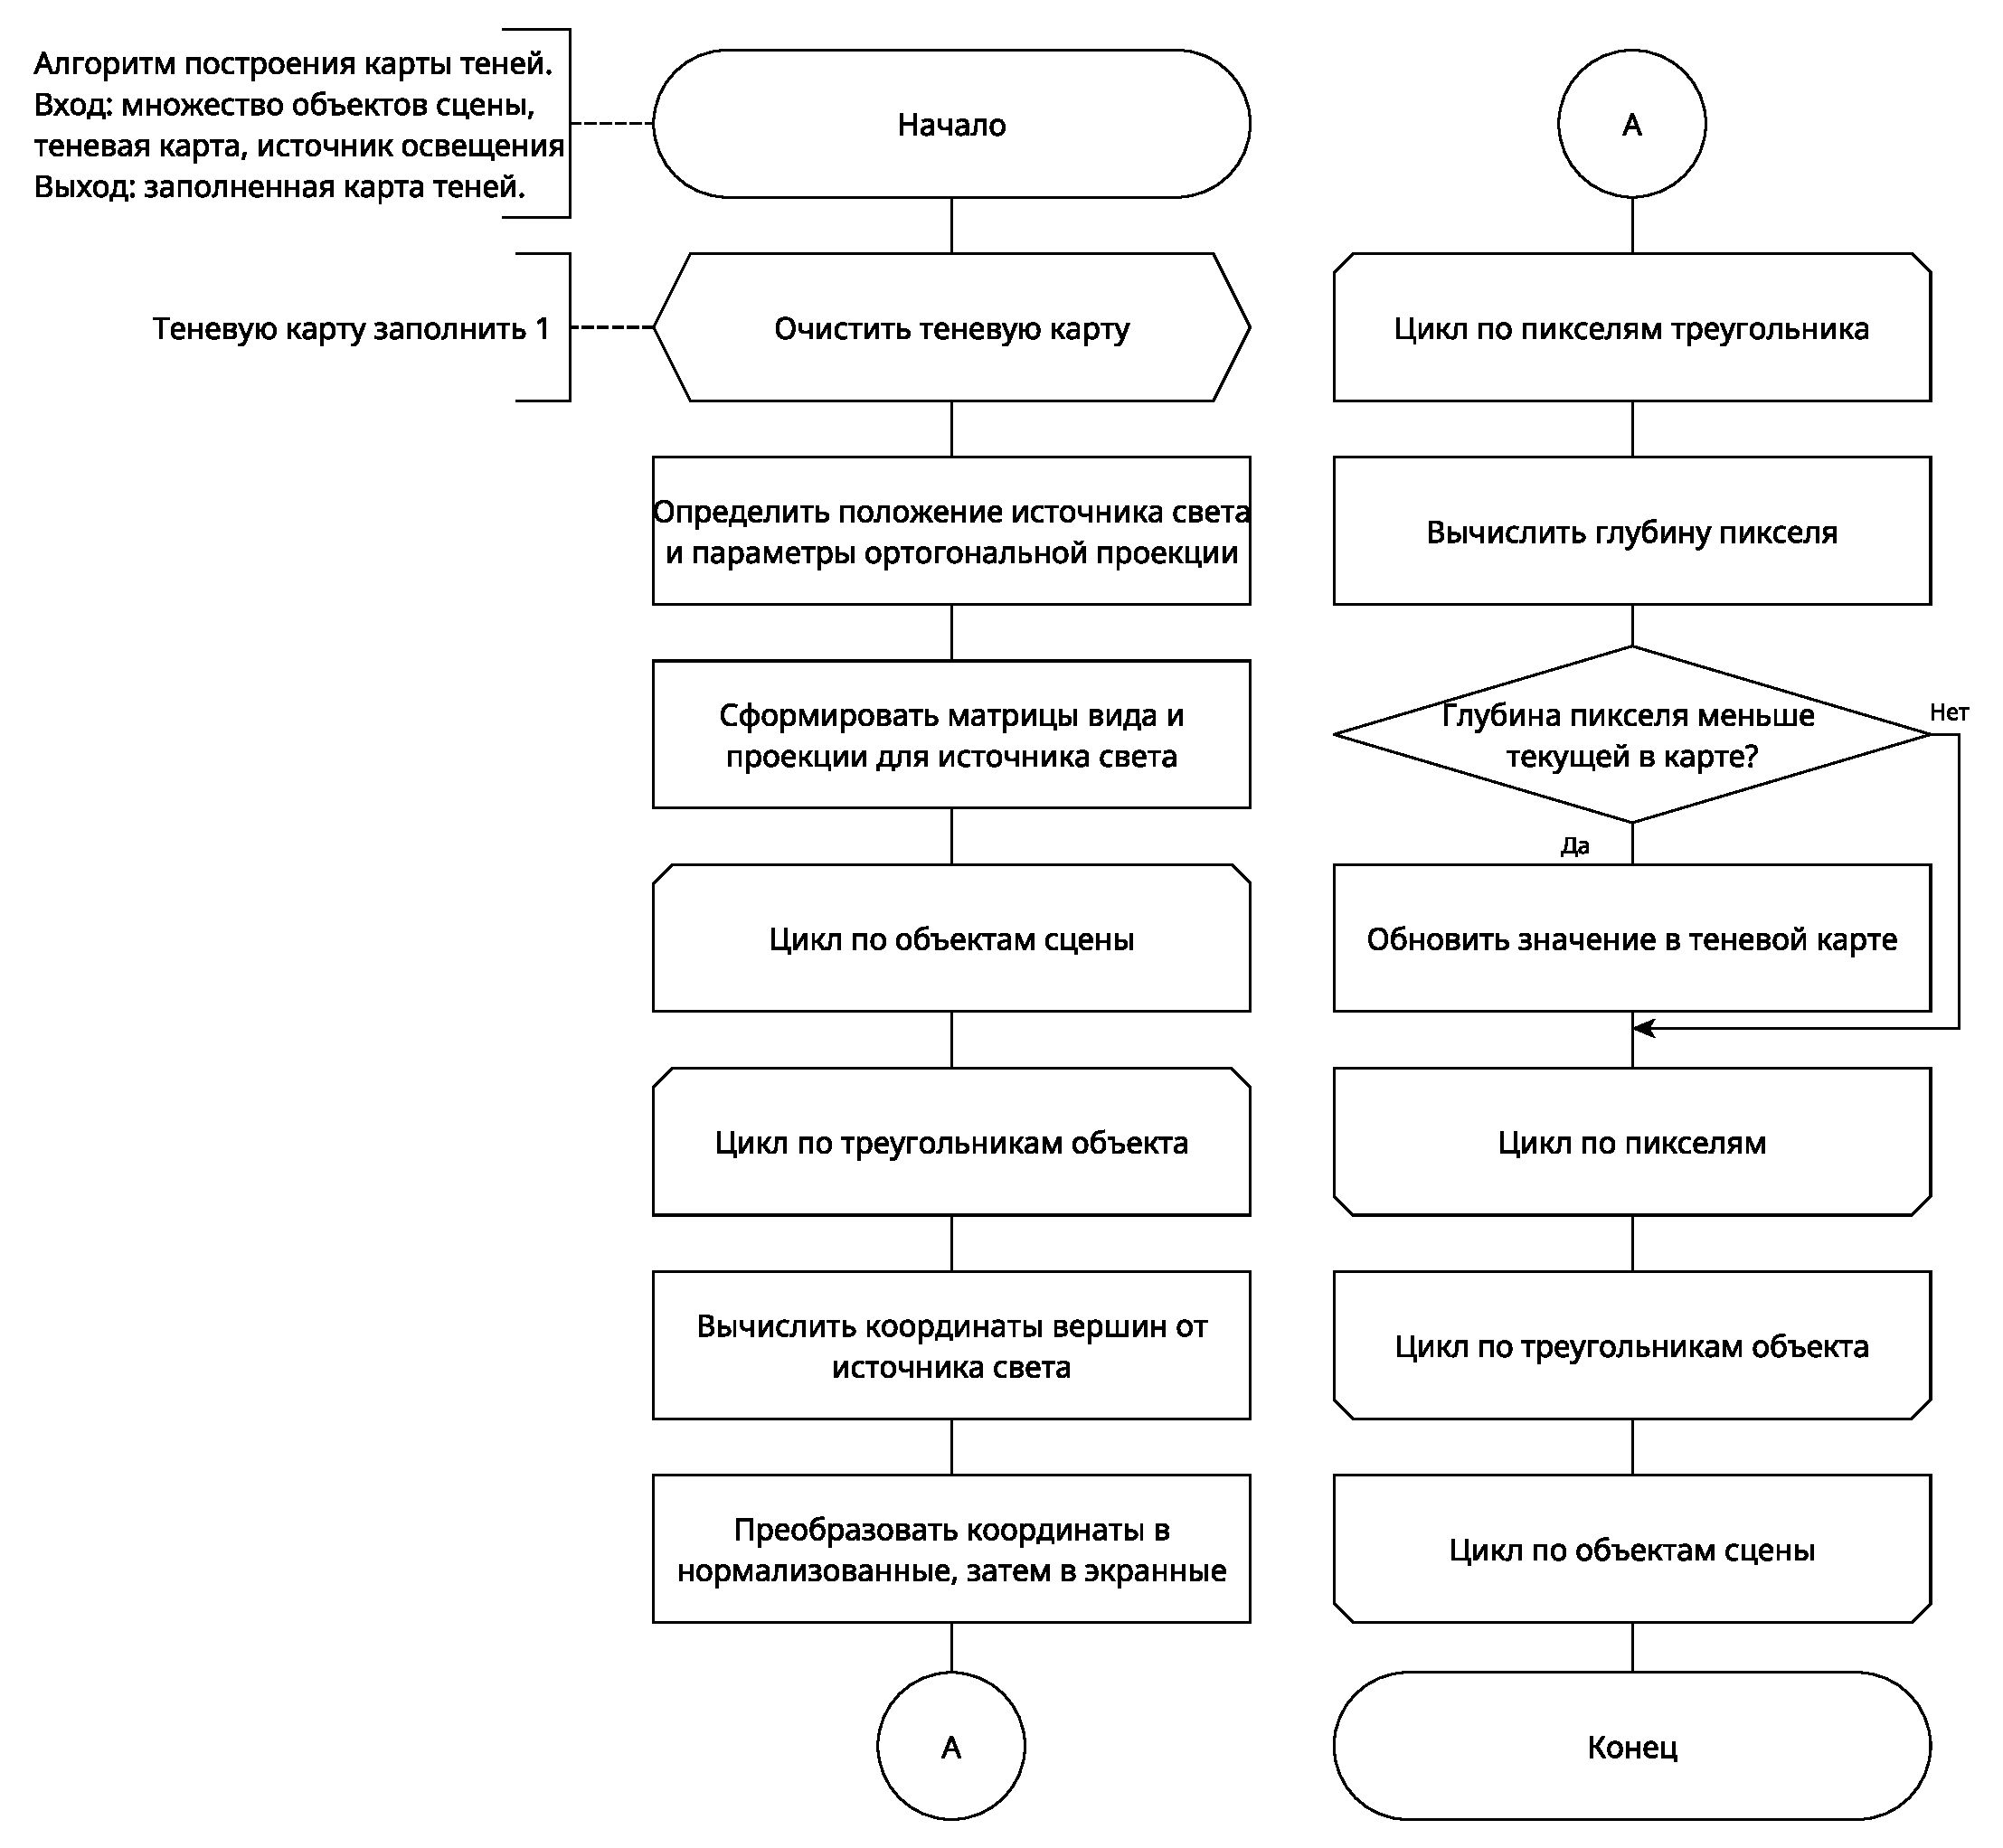
\includegraphics[width=\textwidth]{images/shadow_map.pdf}
    \caption{Схема алгоритма построения теневой карты}
    \label{fig:shadow_map}
\end{figure}


\subsection{Алгоритм растеризации с учётом z-буффера}

Проверка глубины выполняется непосредственно при заполнении каждого треугольника. Для каждого пикселя, покрываемого треугольником, вычисляется интерполированное значение глубины. Если оно меньше текущего значения в z-буфере, обновляются как цвет, так и глубина в соответствующих буферах. Это обеспечивает корректное отображение перекрывающихся ветвей и листьев без предварительной сортировки объектов.

На рисунке~\ref{fig:shadow_map} представлена схема алгоритма растеризации с учётом z-буффера.

\begin{figure}[H]
    \centering
    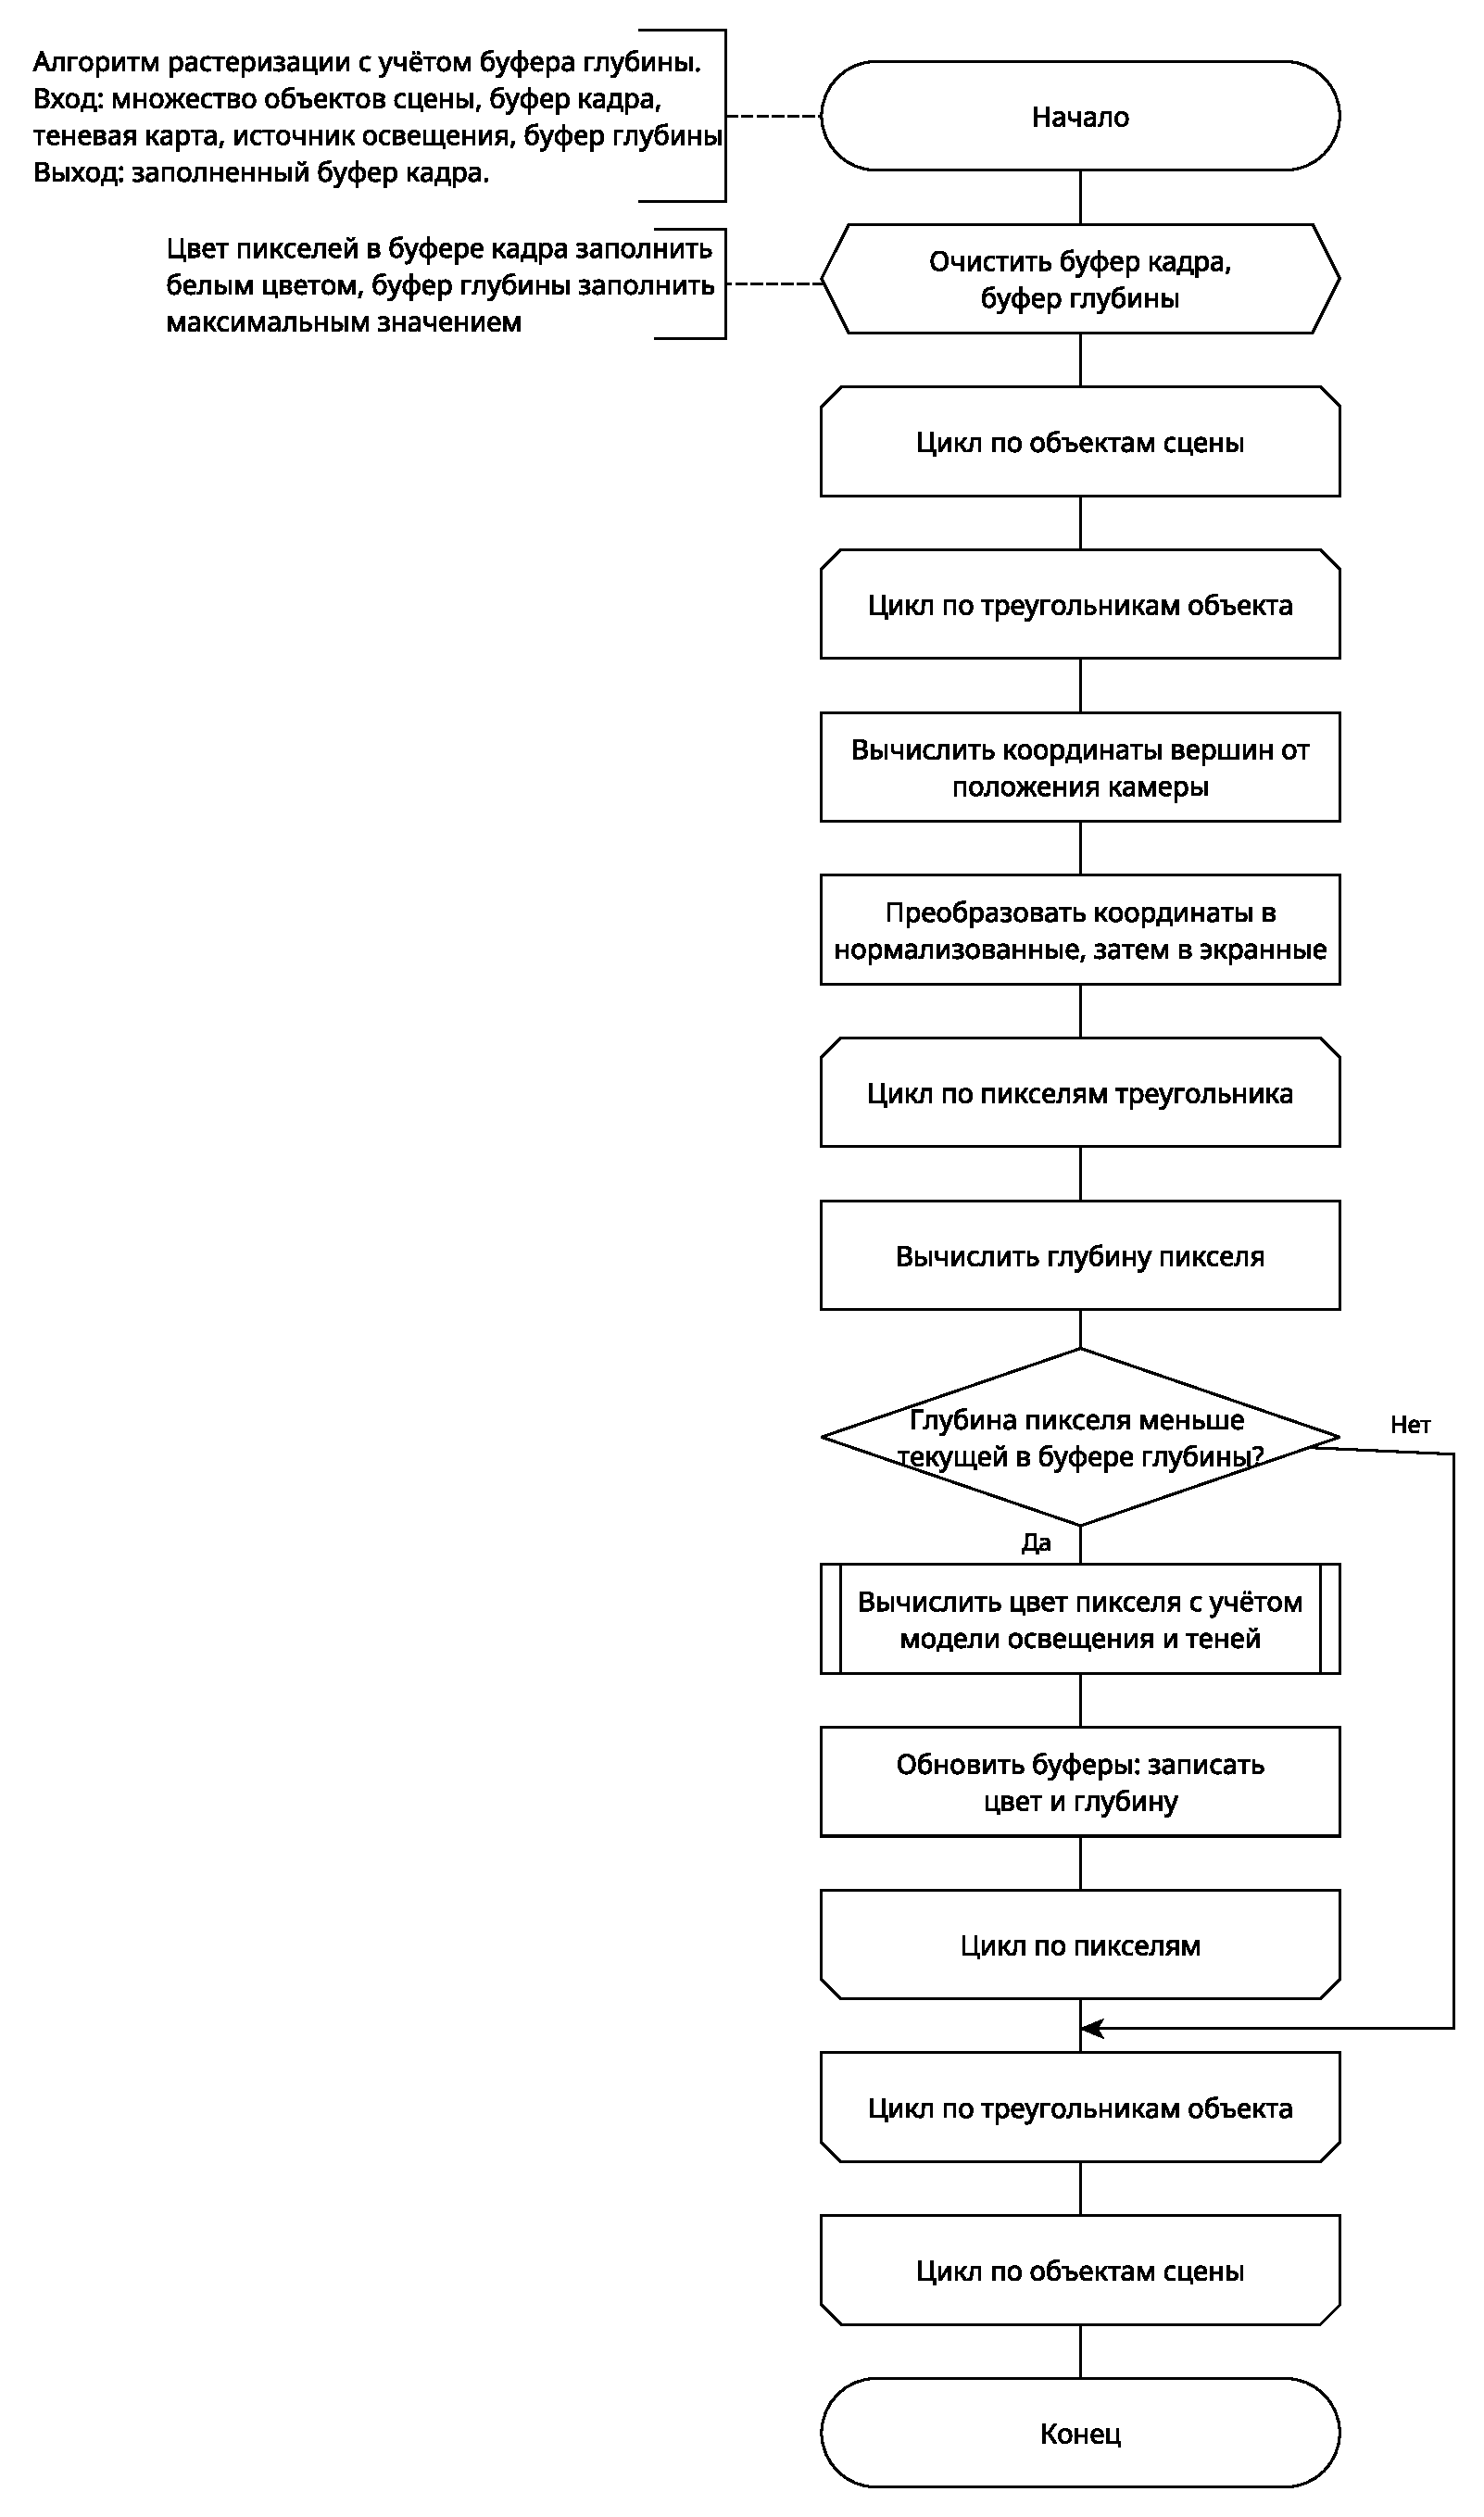
\includegraphics[width=0.77\textwidth]{images/z-buffer.pdf}
    \caption{Схема алгоритма растеризации с учётом z-буффера}
    \label{fig:shadow_map}
\end{figure}

\subsection{Алгоритм модели освещения Блинна-Фонга}

Разработанная модель освещения включает три компонента:
\begin{itemize}
    \item фоновое (ambient) --- равномерное освещение, имитирующее рассеянный свет в сцене;
    \item диффузное (diffuse) --- основной вклад, зависящий от угла между нормалью поверхности и направлением света;
    \item зеркальное (specular) — блик, моделирующий отражение от глянцевых участков.
\end{itemize}

Итоговая формула~\eqref{eq:lighting_total} расчета освещенности в точке:

\begin{equation}
    \label{eq:lighting_total}
    I_{total} = I_{ambient} + I_{diffuse} + I_{specular}
\end{equation}

На рисунке~\ref{fig:lighting_alg} представлена схема алгоритма модели освещения Блинна-Фонга.

\begin{figure}[H]
    \centering
    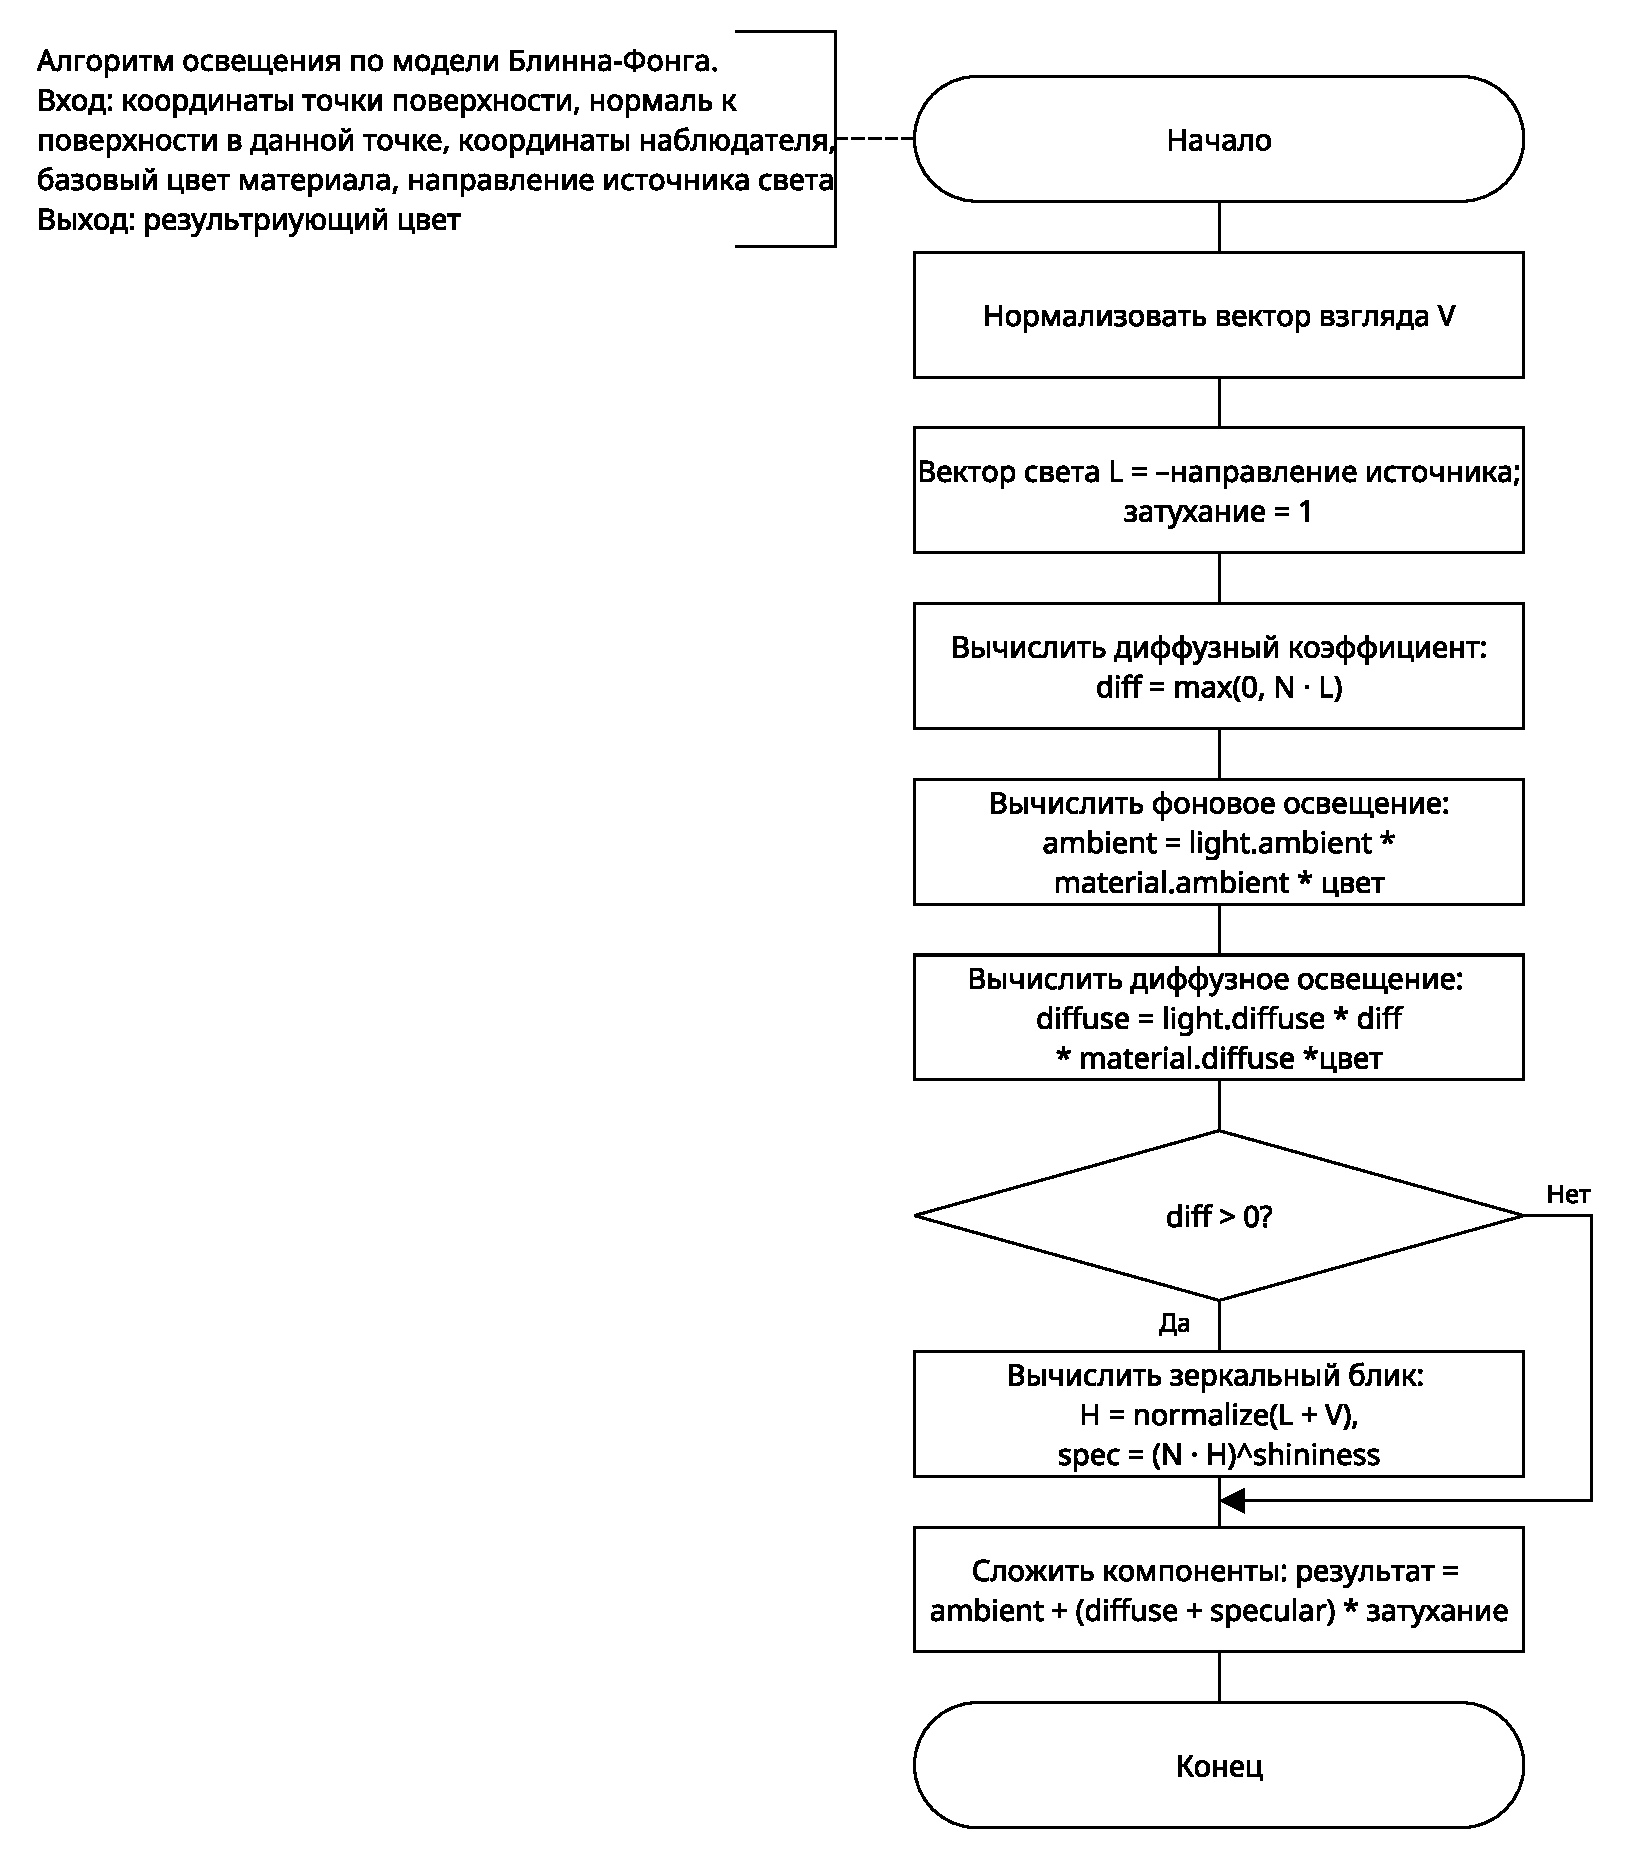
\includegraphics[width=0.96\textwidth]{images/lighting.pdf}
    \caption{Схема алгоритма модели освещения Блинна-Фонга}
    \label{fig:lighting_alg}
\end{figure}


\subsection{Алгоритм генерации структуры дерева на основе L-системы}

Алгоритм принимает на вход аксиому, набор правил продукции и число итераций, после чего последовательно применяет правила к каждому символу строки.

На выходе формируется последовательность команд (таких как \texttt{F}, \texttt{[}, \texttt{+}, \texttt{\&} и др.), которая в дальнейшем интерпретируется трёхмерной черепашьей графикой для построения геометрической модели.

На рисунке~\ref{fig:l-sys_alg} представлена схема данного алгоритма.
\begin{figure}[H]
    \centering
    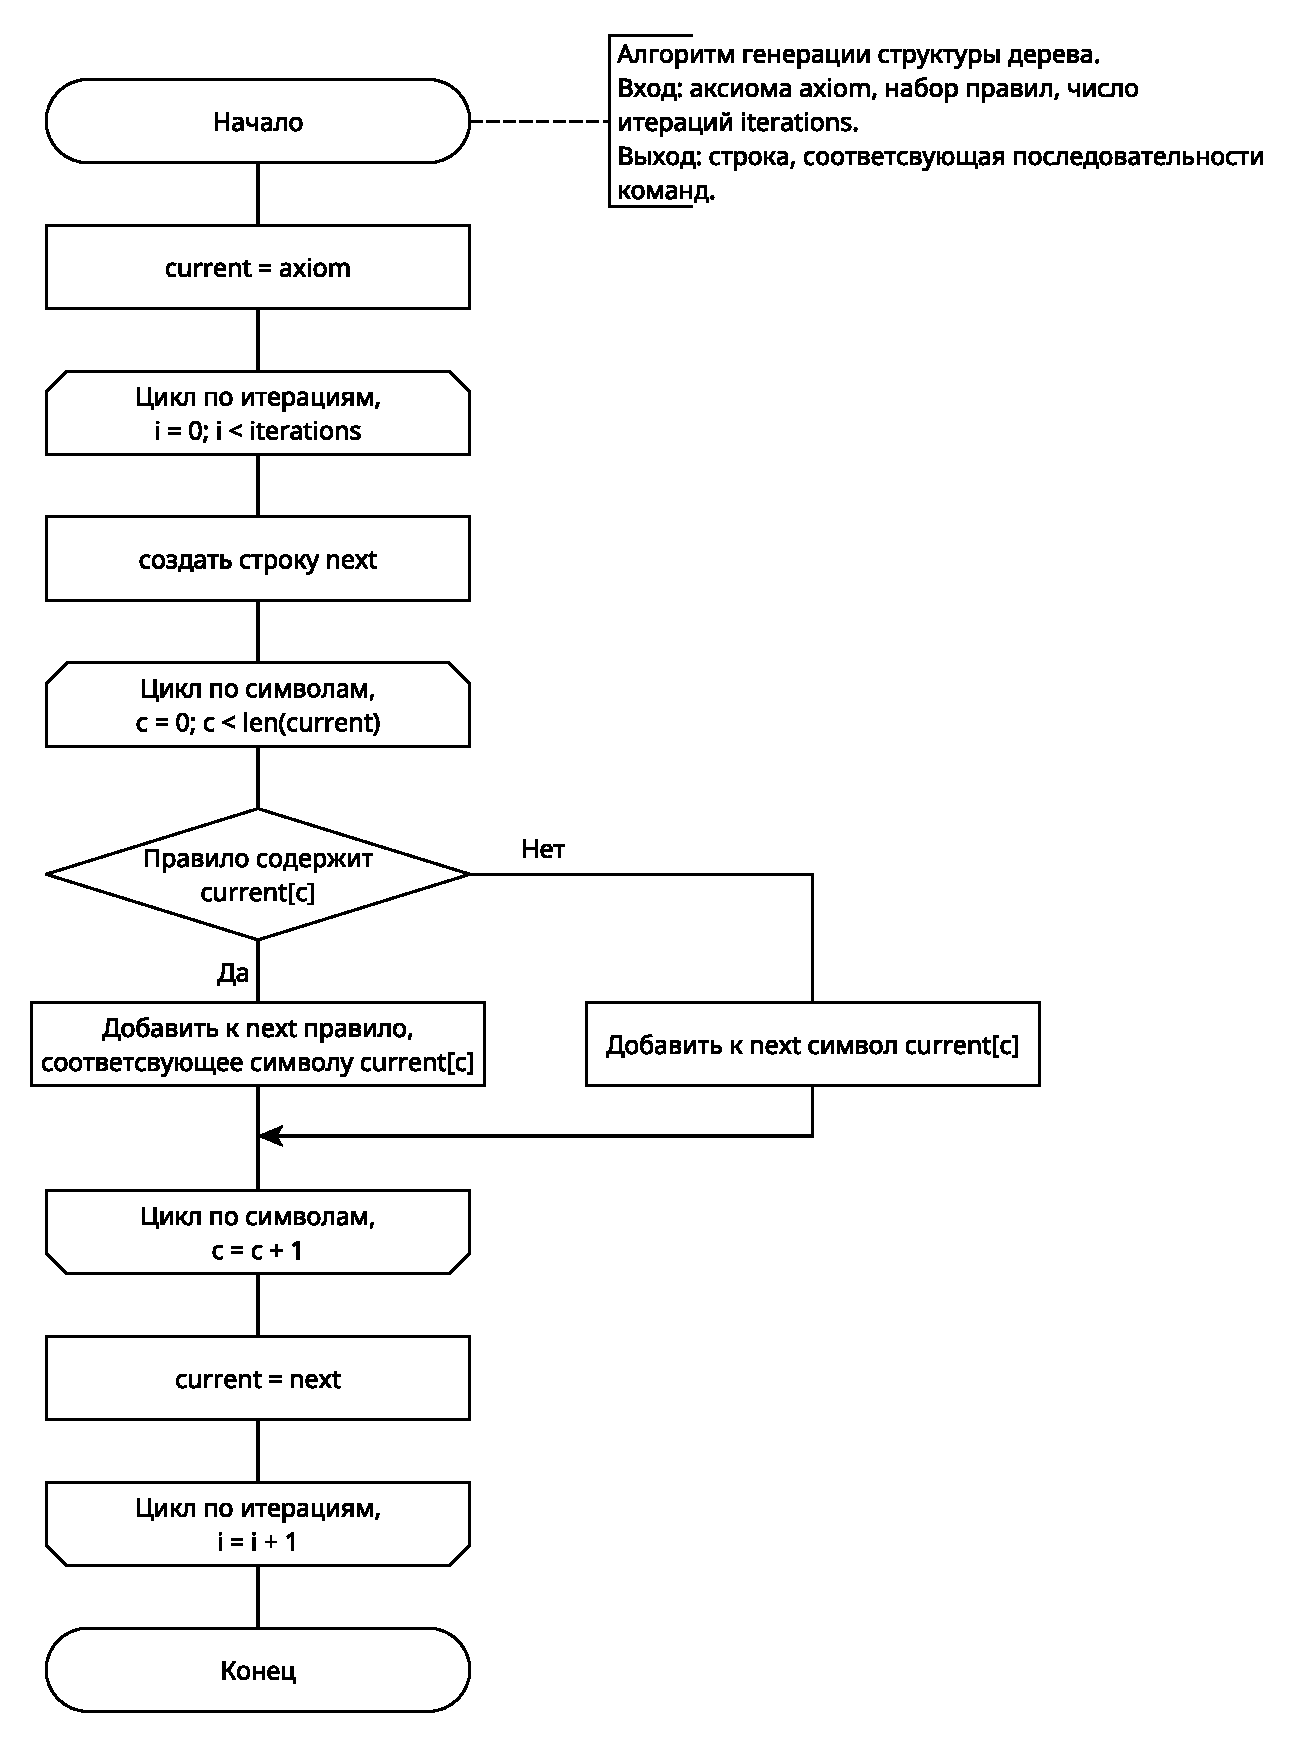
\includegraphics[width=0.9\textwidth]{images/l-sys.pdf}
    \caption{Схема алгоритма генерации структуры дерева на основе заданной L-системы}
    \label{fig:l-sys_alg}
\end{figure}


\section{Вывод}
В конструкторской части было спроектировано программное обеспечение, описаны схемы основных алгоритмов и используемые структуры данных.